\documentclass[11pt,titlepage]{article}
\usepackage{fullpage}
\usepackage{amsmath}
\usepackage{amssymb}
\usepackage{color}
\usepackage{graphicx}
\graphicspath{ {images/} }
\usepackage{tikz}
\usetikzlibrary{shapes,arrows,positioning,calc}
\usepackage{float}
\restylefloat{table}
\usepackage{array}
\tikzset{
    block/.style = {draw, fill=white, rectangle, minimum height=3em, minimum width=3em},
    sum/.style = {draw, fill=white, circle, node distance=1cm},
    input/.style = {draw=none},
    output/.style = {draw=none},
    coord/.style = {coordinate}
}

\author{Rane Brown \\ Kate Schneider}
\title{ECEN 4638: Lab X.1P}
\date{\today}

\begin{document}
\maketitle
\tableofcontents
\listoffigures
\newpage

\section{Description}
    The purpose of this lab is to explore the torsion disc system and experimentally collect data that will help in the design of a proportional controller. The torsion disc system consists of a platform with three discs aligned above a driving motor. There are various configurations for the torsion disc system and this lab will use a basic setup described below. 
    \begin{figure}[h!]
            \centering
            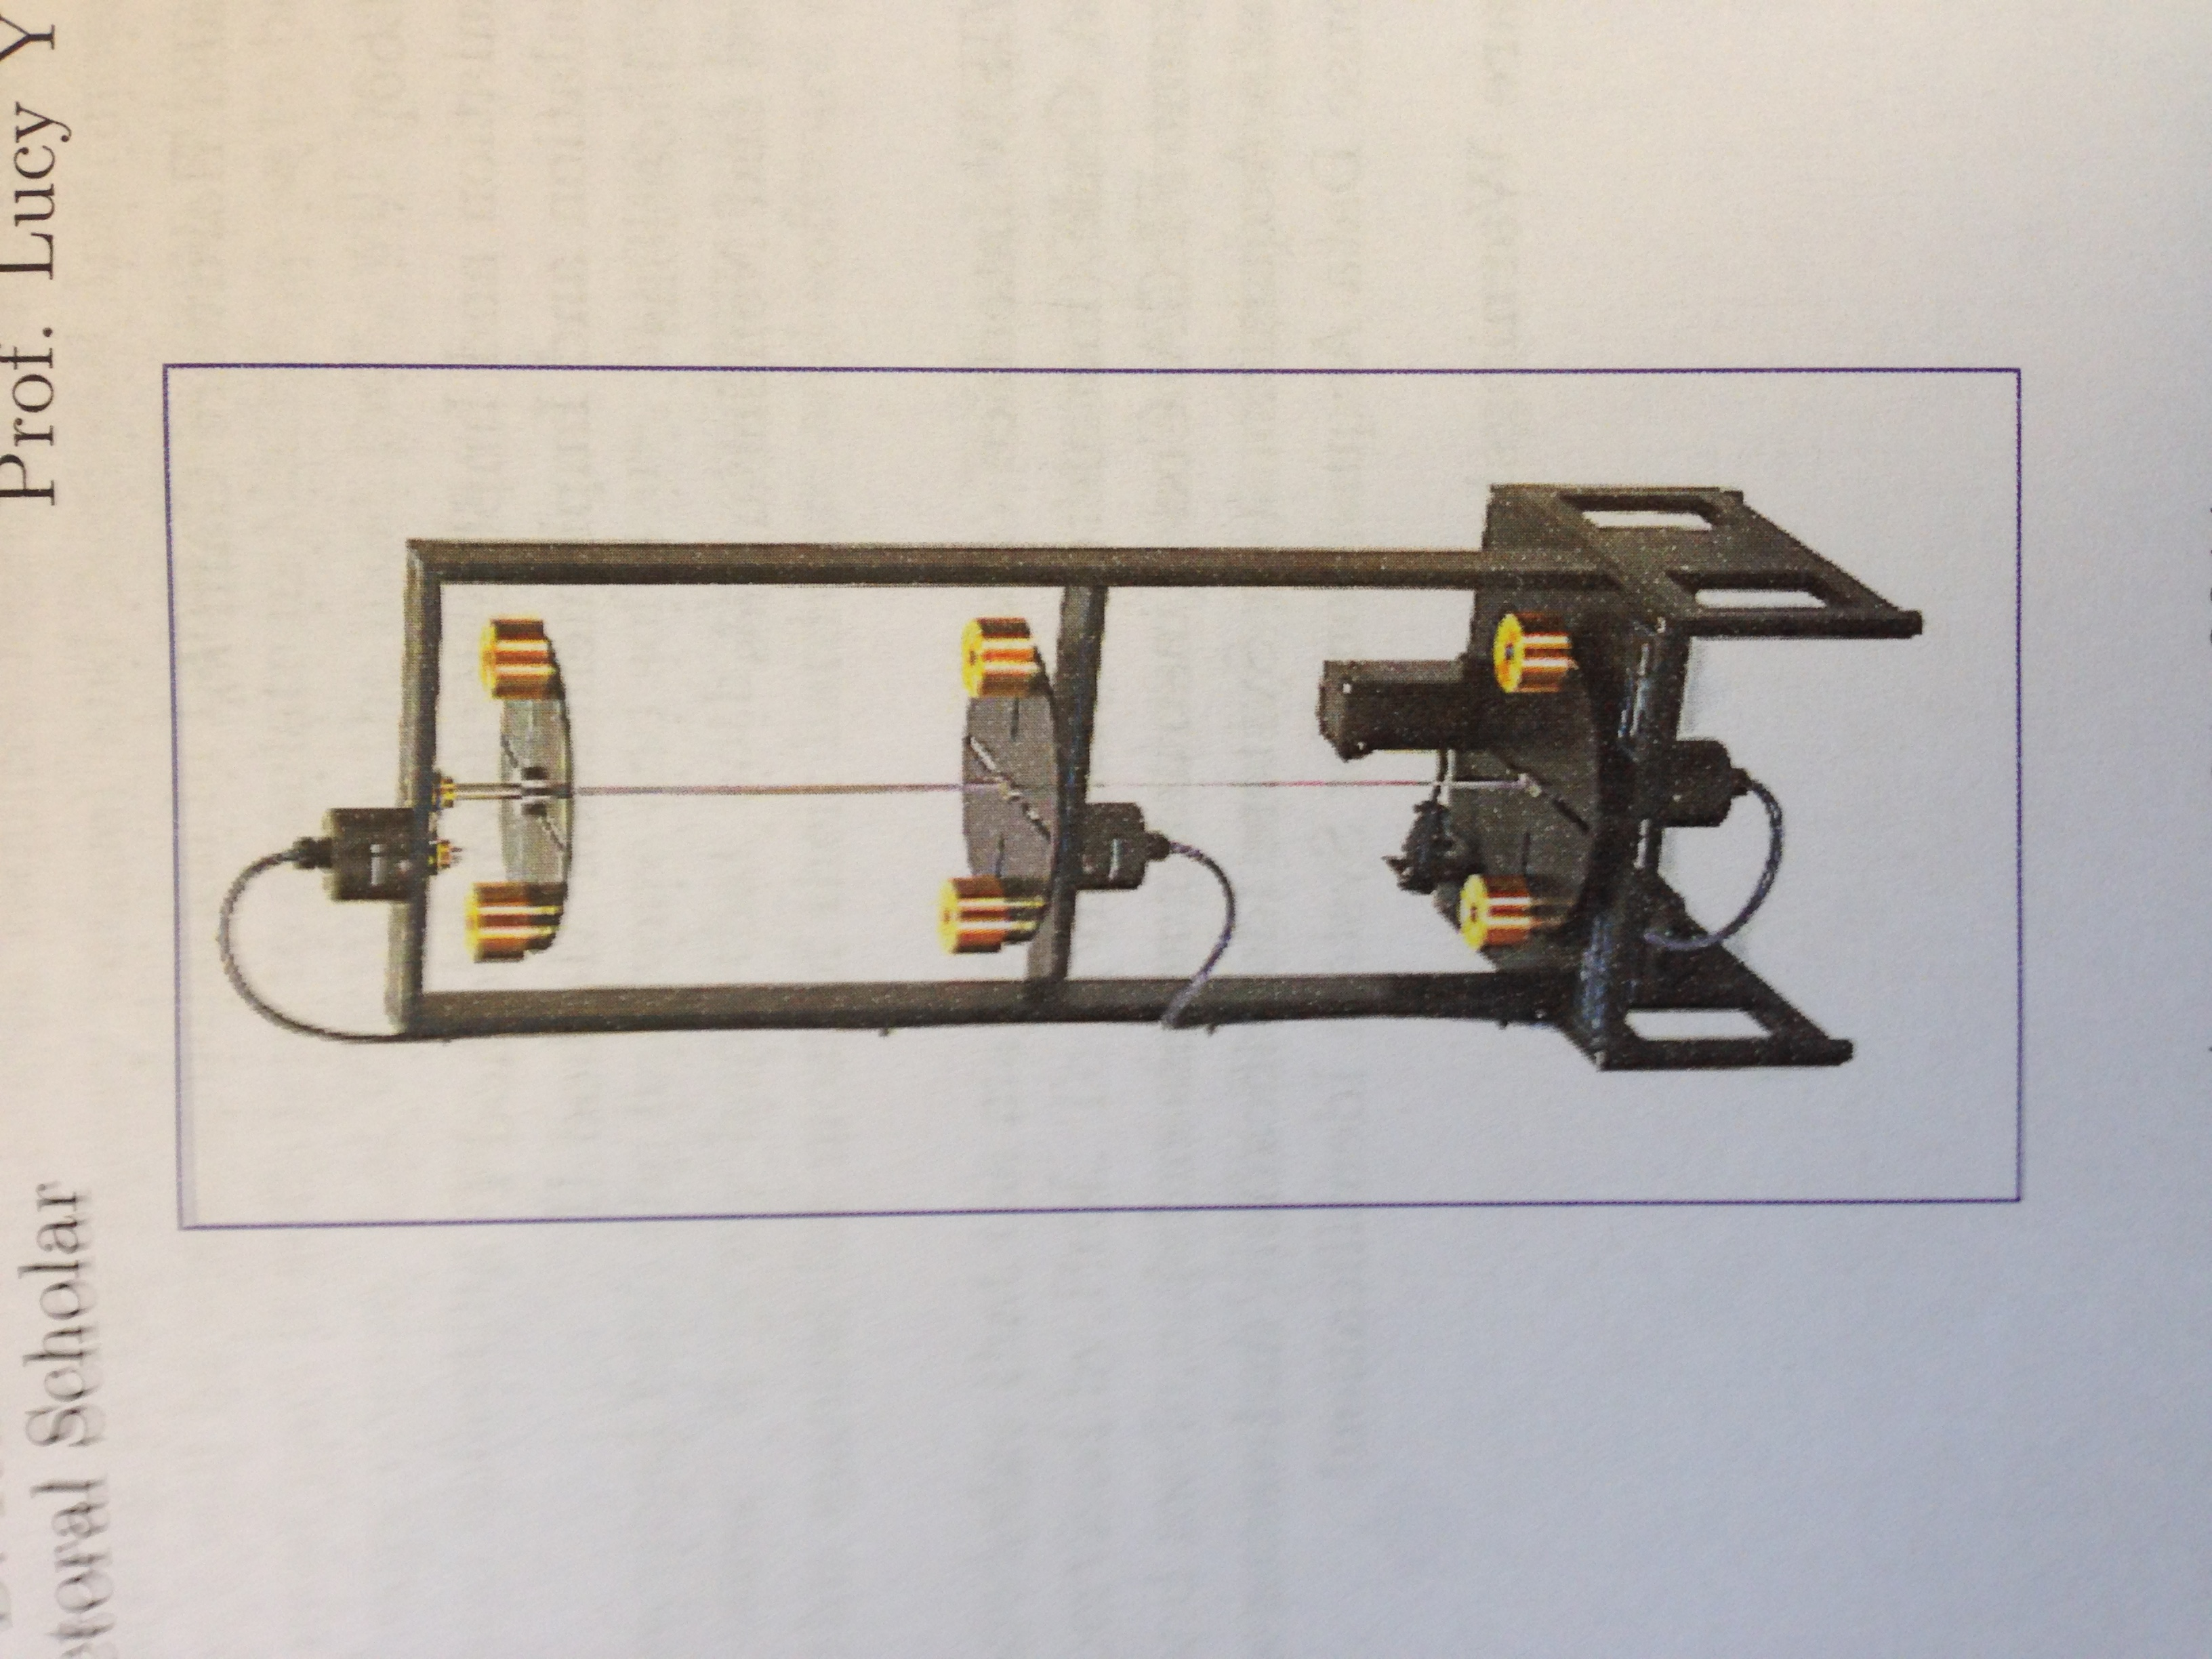
\includegraphics[trim={6cm 0 0 0},clip,angle=-90,origin=c,scale=0.1]{torsionSystem}
            \caption{Torsion Disc System}
            \label{fig:disc_sys}
    \end{figure}

\section{Setup}
    There are three main components that will be necessary for this lab: LabView, Matlab, and the Torsion Disc System. LabView and Matlab do not require any setup as they are installed on all lab computers. On the other hand, the torsion disc system must be configured for proper use. For this experiment the top two discs and any attached weights should be removed. After the weights and discs are removed the system cables can be connected.
    \subsection*{Detailed Steps}
    \begin{enumerate}
        \item loosen allen key screws on all weights attached to the top two discs and remove the weights.
        \item loosen allen key screws on top two discs and detach the discs (each disc is two pieces)
        \item attach all labeled connectors and power lines
    \end{enumerate}

\section{LabView Intro}
    LabView is a high level program that will be used to control the torsion disc system. Data from the system will also be collected using LabView. The general idea is to build a block diagram of the system with appropriate input and output values as well as a configurable controller. In order to understand the operation of LabView it is useful to create a demo system before beginning work on the Torsion Disc system.
    \subsection{Simulation Loop}
        Figure \ref{fig:sim_intro} shows a simulation loop that was created in LabView. Transfer function blocks were used for the vehicle and controller while the reference and disturbance inputs use lookup tables. The output of the system is written to an external file.
        \begin{figure}[h!]
            \centering
            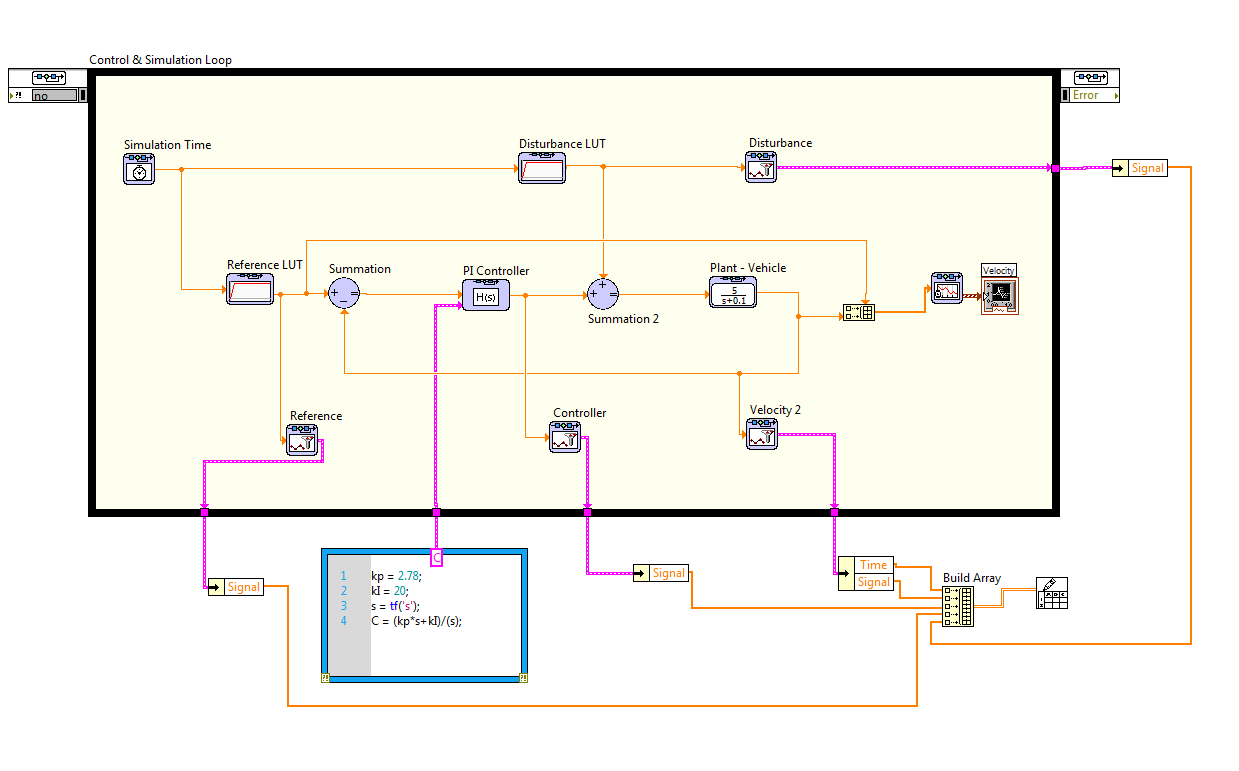
\includegraphics[scale=.5]{labviewIntro}
            \caption{LabView Intro Model}
            \label{fig:sim_intro}
        \end{figure}
    \subsection{Controller Results}
        The created simulation was run with various values of $K_p$ and $K_I$ and the output was observed and recorded. The collected results from the LabView simulations were then taken and compared to the Simulink model used in LabX. As seen in figure \ref{fig:kp1} and figure \ref{fig:kp5KI10}, the results from LabView and simulink are comparable.
        \begin{figure}[h!]
            \centering
            \begin{minipage}{.5\textwidth}
                \centering
                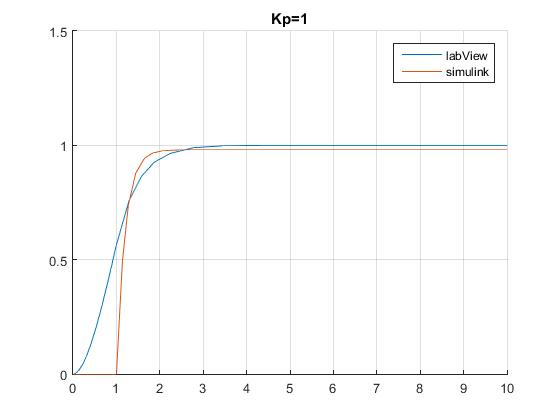
\includegraphics[scale=.4]{Kp1}
                \caption{P Controller $K_p=1$}
                \label{fig:kp1}
            \end{minipage}%
            \begin{minipage}{.5\textwidth}
                \centering
                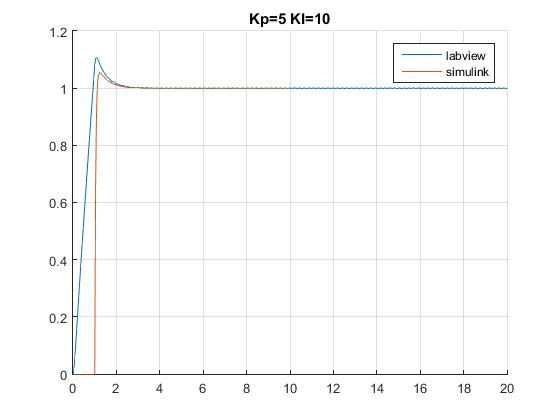
\includegraphics[scale=.4]{Kp5KI10}
                \caption{PI Controller $K_p=5$ $K_I=10$}
                \label{fig:kp5KI10}
            \end{minipage}%
        \end{figure}    
    \subsection{Disturbance} 
        As a final experiment a disturbance was introduced to the LabView model that simulates a hill. The $P$ and $P_I$ values were chosen in order to produce a fast response with a small amount of overshoot and a reasonable settle time. In this case, values of $K_I=20$ and $K_I=60$ worked well. The results of this experiment are shown in figure \ref{fig:resp_dist}.
        \begin{figure}[h!]
            \centering
            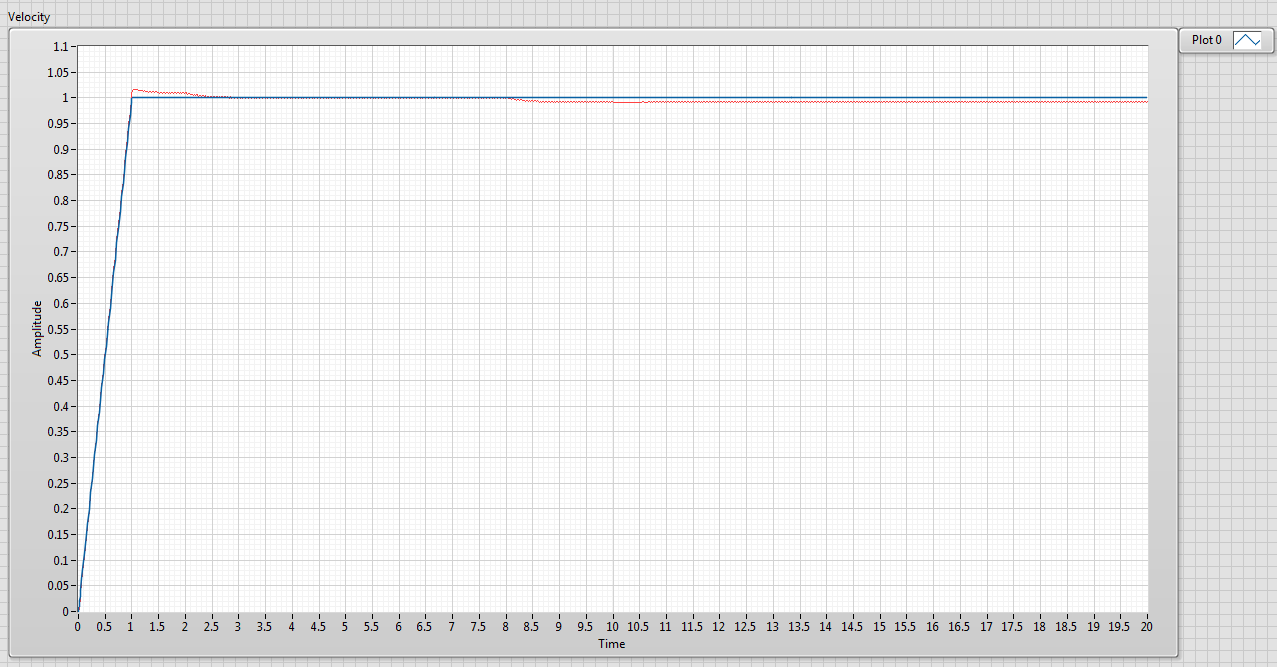
\includegraphics[scale=.4]{disturbance}
            \caption{Response with disturbance}
            \label{fig:resp_dist}
        \end{figure}

\section{Data Collection}
    To create a LTI model for the Torsion Disc system it was necessary to collect data that could be used to estimate system parameters. A LabView model was used to control the system and collect necessary data. The LabView model shown in figure \ref{fig:labview_sys} was provided for this experiment and can be found on the ITLL share drive. Two experiments were conducted to collect the needed data. \emph{NOTE: equations are found in section \ref{sec:LTI}.}
    \begin{figure}[h!]
            \centering
            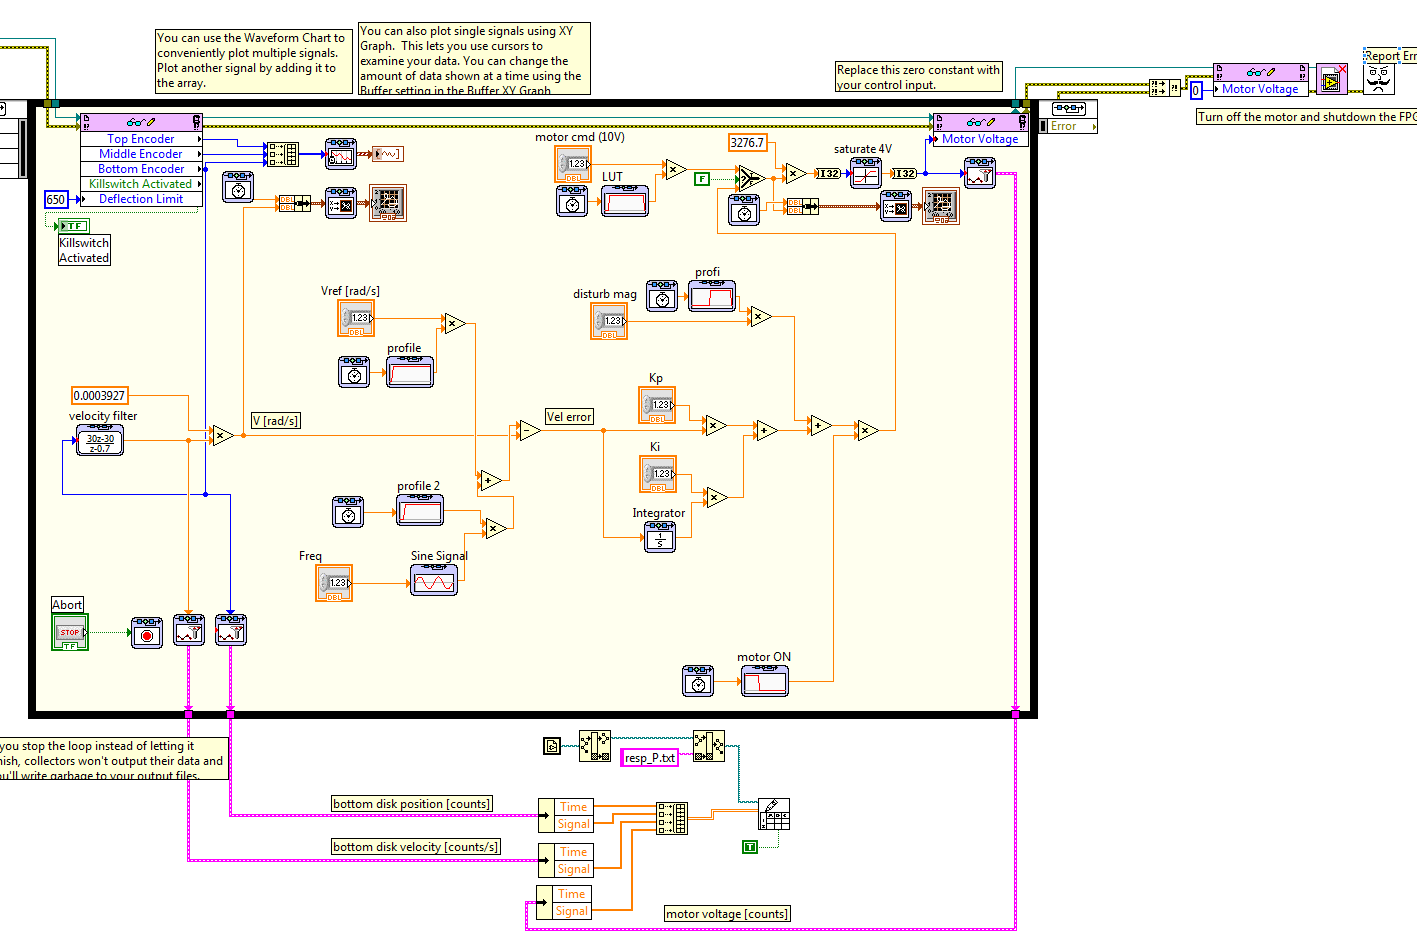
\includegraphics[trim={0 0 10cm 0},clip,scale=0.4]{labviewModel}
            \caption{LabView Control System}
            \label{fig:labview_sys}
    \end{figure}
    \subsection{No motor voltage}
        The first experiment was conducted with no power connected to the Torsion Disc motor. This was done in order to eliminate some of the parameters from the LTI model in order to estimate the value of $c$. Data was collected for three different weight positions as shown in table \ref{table:weight_pos}. Each weight position gives a different inertia value for the system. The data is collected by first selecting a weight position and then manually spinning the disc by hand. \emph{If only 2 weights are used they must be located along the hub split line.}
    \subsection*{Steps}
        \begin{enumerate}
            \itemsep0em 
            \item set the weights to a desired radius on the lower disc
            \item make sure the bolts holding the weights are firmly tightened
            \item begin data collection in LabView
            \item manually spin the disc and allow it to come to a stop
            \item data is saved as a text file
            \item change filename to reflect the weight position
        \end{enumerate}
        \begin{table}[h!]
            \centering
            \begin{tabular}{|m{4cm}|m{3cm}|m{3cm}|} 
                \hline
                Number of weights & Radius & Inertia $J$ \\ 
                \hline
                4 & 9 cm & 0.0192 \\
                \hline
                4 & 7.5 cm & 0.0143\\
                \hline
                2 & 4.5 cm & 0.0043 \\
                \hline
            \end{tabular}
            \caption{Weights and Position} \label{table:weight_pos}
        \end{table}
    \subsection{Powered Torsion Disc System}
    The second data collection experiment was conducted with the power connected to the Torsion Disc system. In this case the values of various system parameters are adjusted in LabView while the weights remain in the same position. The collected data is then used to create a proportional controller.
    \subsection*{Steps}
        \begin{enumerate}
            \itemsep0em 
            \item set reference speed to 3.14 rad/sec
            \item set disturbance to 0
            \item set $K_p$ to 1
            \item adjust experiment length to 12 seconds in order to collect data as the system comes to a stop
            \item \textbf{Ensure there is someone with their finger on the power of button in case the system goes unstable}
            \item turn the power on
            \item press the run button in LabView, data is saved as a text file
            \item rename file to reflect parameter values
            \item repeat for the values listed in table \ref{table:data_param}
        \end{enumerate}
        \begin{table}[H]
            \centering
            \begin{tabular}{|m{4cm}|m{3cm}|m{3cm}|} 
                \hline
                Reference rad/sec & $K_p$ & Disturbance \\ 
                \hline
                3.14 & 1,5,10 & 0\\
                \hline
                3.14 & 1,5,10 & 1\\
                \hline
                6.28 & 1,5,10 & 0 \\
                \hline
                6.28 & 1,5,10 & 1 \\
                \hline
            \end{tabular}
            \caption{Data Collection Parameters} \label{table:data_param}
        \end{table}
        \subsection{Observations}
        While performing the torsion disc experiment with motor power on, it was found that too large a gain $k_p$ produced undesired effects in the system. When $k_p$ was increased above 15, the motor voltage became very noisy, and the system began to show signs of instability. A $k_p$ value of 10 was found to produce less noise in the motor while still providing a large gain for the system. 

\section{LTI Model} \label{sec:LTI}
    The Torsion Disc system can be modeled as an LTI system with the below equation.
    \begin{equation} \label{eq:lti}
        J\dot{\omega}+c\omega=k_hu
    \end{equation}
    Where $J=\mbox{ total system inertia}$, $\omega=\mbox{ velocity rad/sec}$, $c=\mbox{ system drag}$, $k_h=\mbox{ hardware gain}$, $u=\mbox{ reference}$.

    \subsection{Calculating parameter $J$}
        The inertia of the system can be calculated from the system parameters (inertia of the torsion disk, $J_{disk}$, inertia of the motor, $J_{motor}$, and inertia of the weights, $J_{weight}$) as follows:
        $$J_{disk}=0.0019$$
        $$J_{motor}=0.0005$$
        \begin{equation}
            J_{weight}=\sum\limits_{i=1}^{N} \frac{1}{2}mr^2 + mR^2\\
        \end{equation}
        Thus the total inertia is:
        \begin{align}
            J_{tot}&=J_{disc}+J_{motor}+J_{weight}\nonumber\\
            J_{tot}&=0.0019+0.0005+\sum\limits_{i=1}^{N} \frac{1}{2}mr^2 + mR^2
        \end{align}
    \subsection{Estimating parameter $c$}
    From the LTI model above, system drag $c$ can be estimated as follows:
        \begin{align}
            \omega(t)&=e^{\frac{-c}{J}t_1}\omega(t_0)\nonumber\\
            ln\left( \frac{\omega(t_1)}{\omega(t_0)}\right)&=\frac{-c}{J}(t_1-t_0)\nonumber\\
            c&=\frac{-Jln\left(\frac{\omega(t_1)}{\omega(t_0)}\right)}{t_1-t_0}\label{eq:find_c}
        \end{align}
        To estimate $c$ from collected data, the natural logarithm of angular velocity $\omega$ is plotted against time. A reasonably straight part of the curve is chosen, from time $t_0$ to time $t_1$. The total system inertia and angular velocities $\omega(t_0)$ and $\omega(t_1)$ are then used with equation~\ref{eq:find_c} to estimate system drag $c$. Plots of filtered and unfiltered angular velocity data were analyzed, and filtering was found not to significantly affect the plot or $c$ value obtained from the data. Thus, the unfiltered velocity data alone was used to estimate $c$. This was repeated for several experiments and $c$ values were averaged, resulting in a $c$ value of 
        \begin{equation}
            c=0.0079\nonumber
        \end{equation}
        A sample plot is shown below for $k_p=1$ and a reference input of $\omega_{ref}=6.28$ rad/s. The relatively linear section from $t_0=7.5s$ to $t_1=8.5s$ was chosen for estimating $c$. Choosing a time period when angular velocity was well above 0 reduced the influence of motor poles on the system and the estimation of $c$.
        
        \begin{figure}[h!]
            \centering
            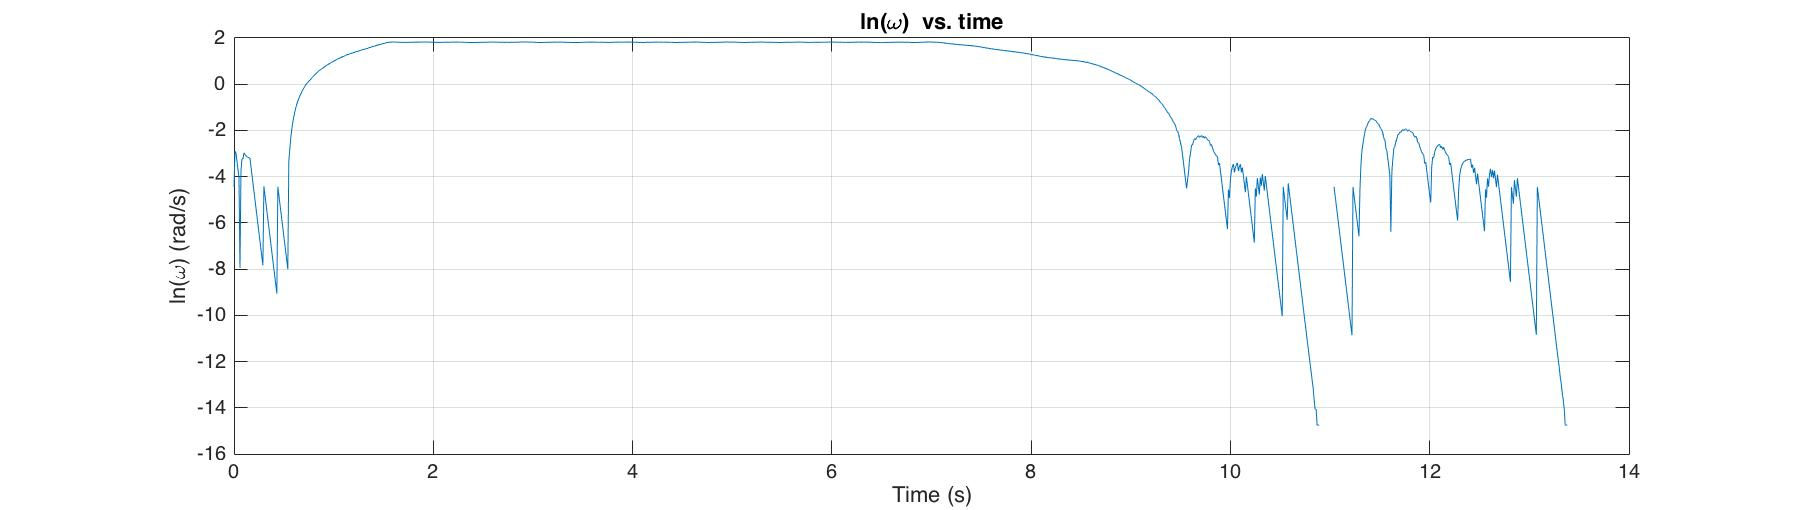
\includegraphics[trim={6cm 0 0 0},clip,angle=0,origin=c,scale=0.3]{lnw_vs_time}
            \caption{ln($\omega$) vs. time}
            \label{fig:lnw_vs_time}
        \end{figure}
    \subsection{Estimating parameter $k$}
        When angular acceleration $\dot{\omega}=0$, the equation describing our LTI system becomes
        \begin{align}
            c\omega=k_hu\nonumber\\
            k_h=\frac{\omega}{u}c\label{eq:k_h}
        \end{align}
        Hardware gain $k_h$ can be estimated from the above equation, where $c$ is calculated as in the previous section, $\omega$ is the average rotational velocity of the system, and $u$ is the average motor voltage when the system is running at a constant speed. Parameters $\omega$ and $u$ were plotted against time to determine when the system was at a constant speed. $\omega$ and $u$ were averaged over the chosen time period and equation \ref{eq:k_h} was then used to estimate $k_h$. This was repeated for several experiments and $\omega$ and $u$ values were averaged. The resulting $k_h$ value is
        \begin{equation}
            k_h=0.3598\nonumber
        \end{equation}
        This value for $k_h$ is very close to the nominal value calculated from system parameters 
        \begin{align*}
            &\mbox{\emph{Pulley Magnification}}                 &       k_p&=3      &   &\frac{Nm}{Nm}\\
            &\mbox{\emph{Drive Motor Torque Constant}}          &       k_m&=0.086  &   &\frac{Nm}{Nm}\\
            &\mbox{\emph{Drive Motor Amplifier Current Gain}}   &       k_a&=1.5    &   &\frac{A}{V}
        \end{align*}
        \begin{align*}
            k_{h nominal}&=k_pk_mk_a\\
            k_{h nominal}&=0.387
        \end{align*}
        Sample plots used to evaluate average rotational velocity $\omega$ and average motor voltage $u$ are shown below. The time period from $t_0=2$ seconds to $t_1=7$ seconds was used to calculate average $\omega$ and $u$.
        \begin{figure}[H]
            \centering
            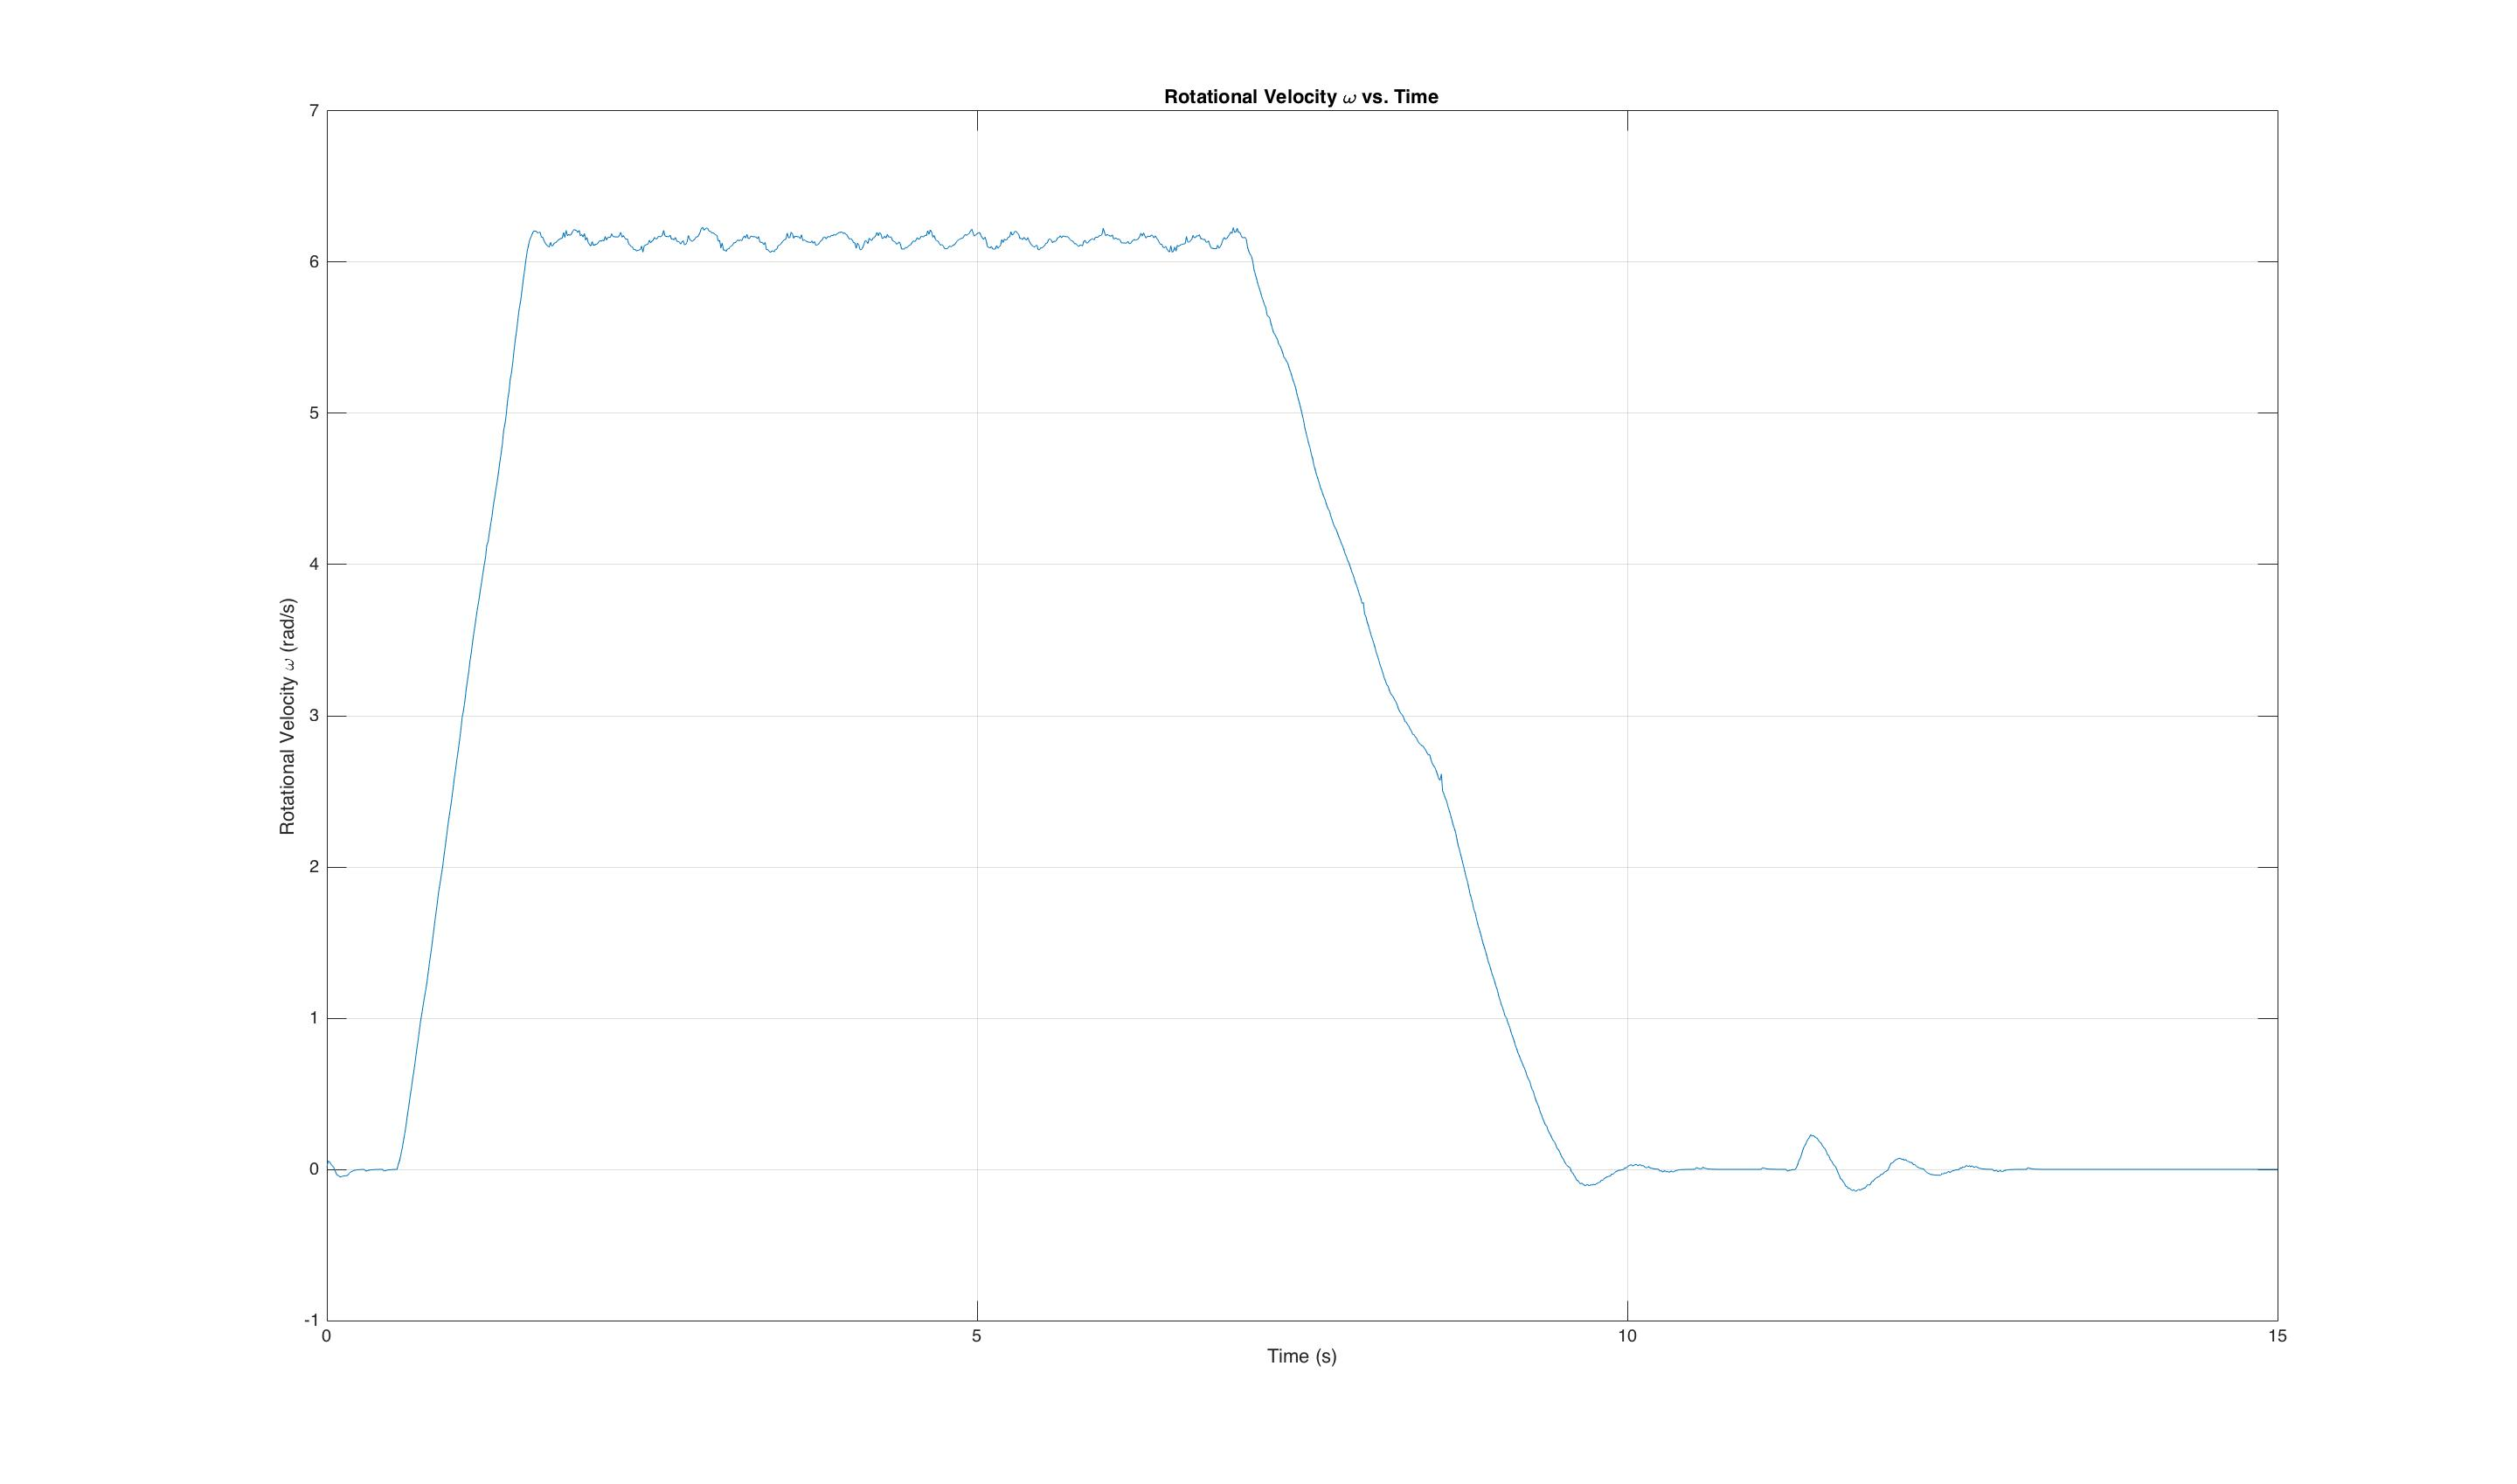
\includegraphics[scale=0.1]{w_vs_time}
            \caption{Rotational Velocity $\omega$ vs. Time}
            \label{fig:w_vs_time}
        \end{figure}
        \begin{figure}[H]
            \centering
            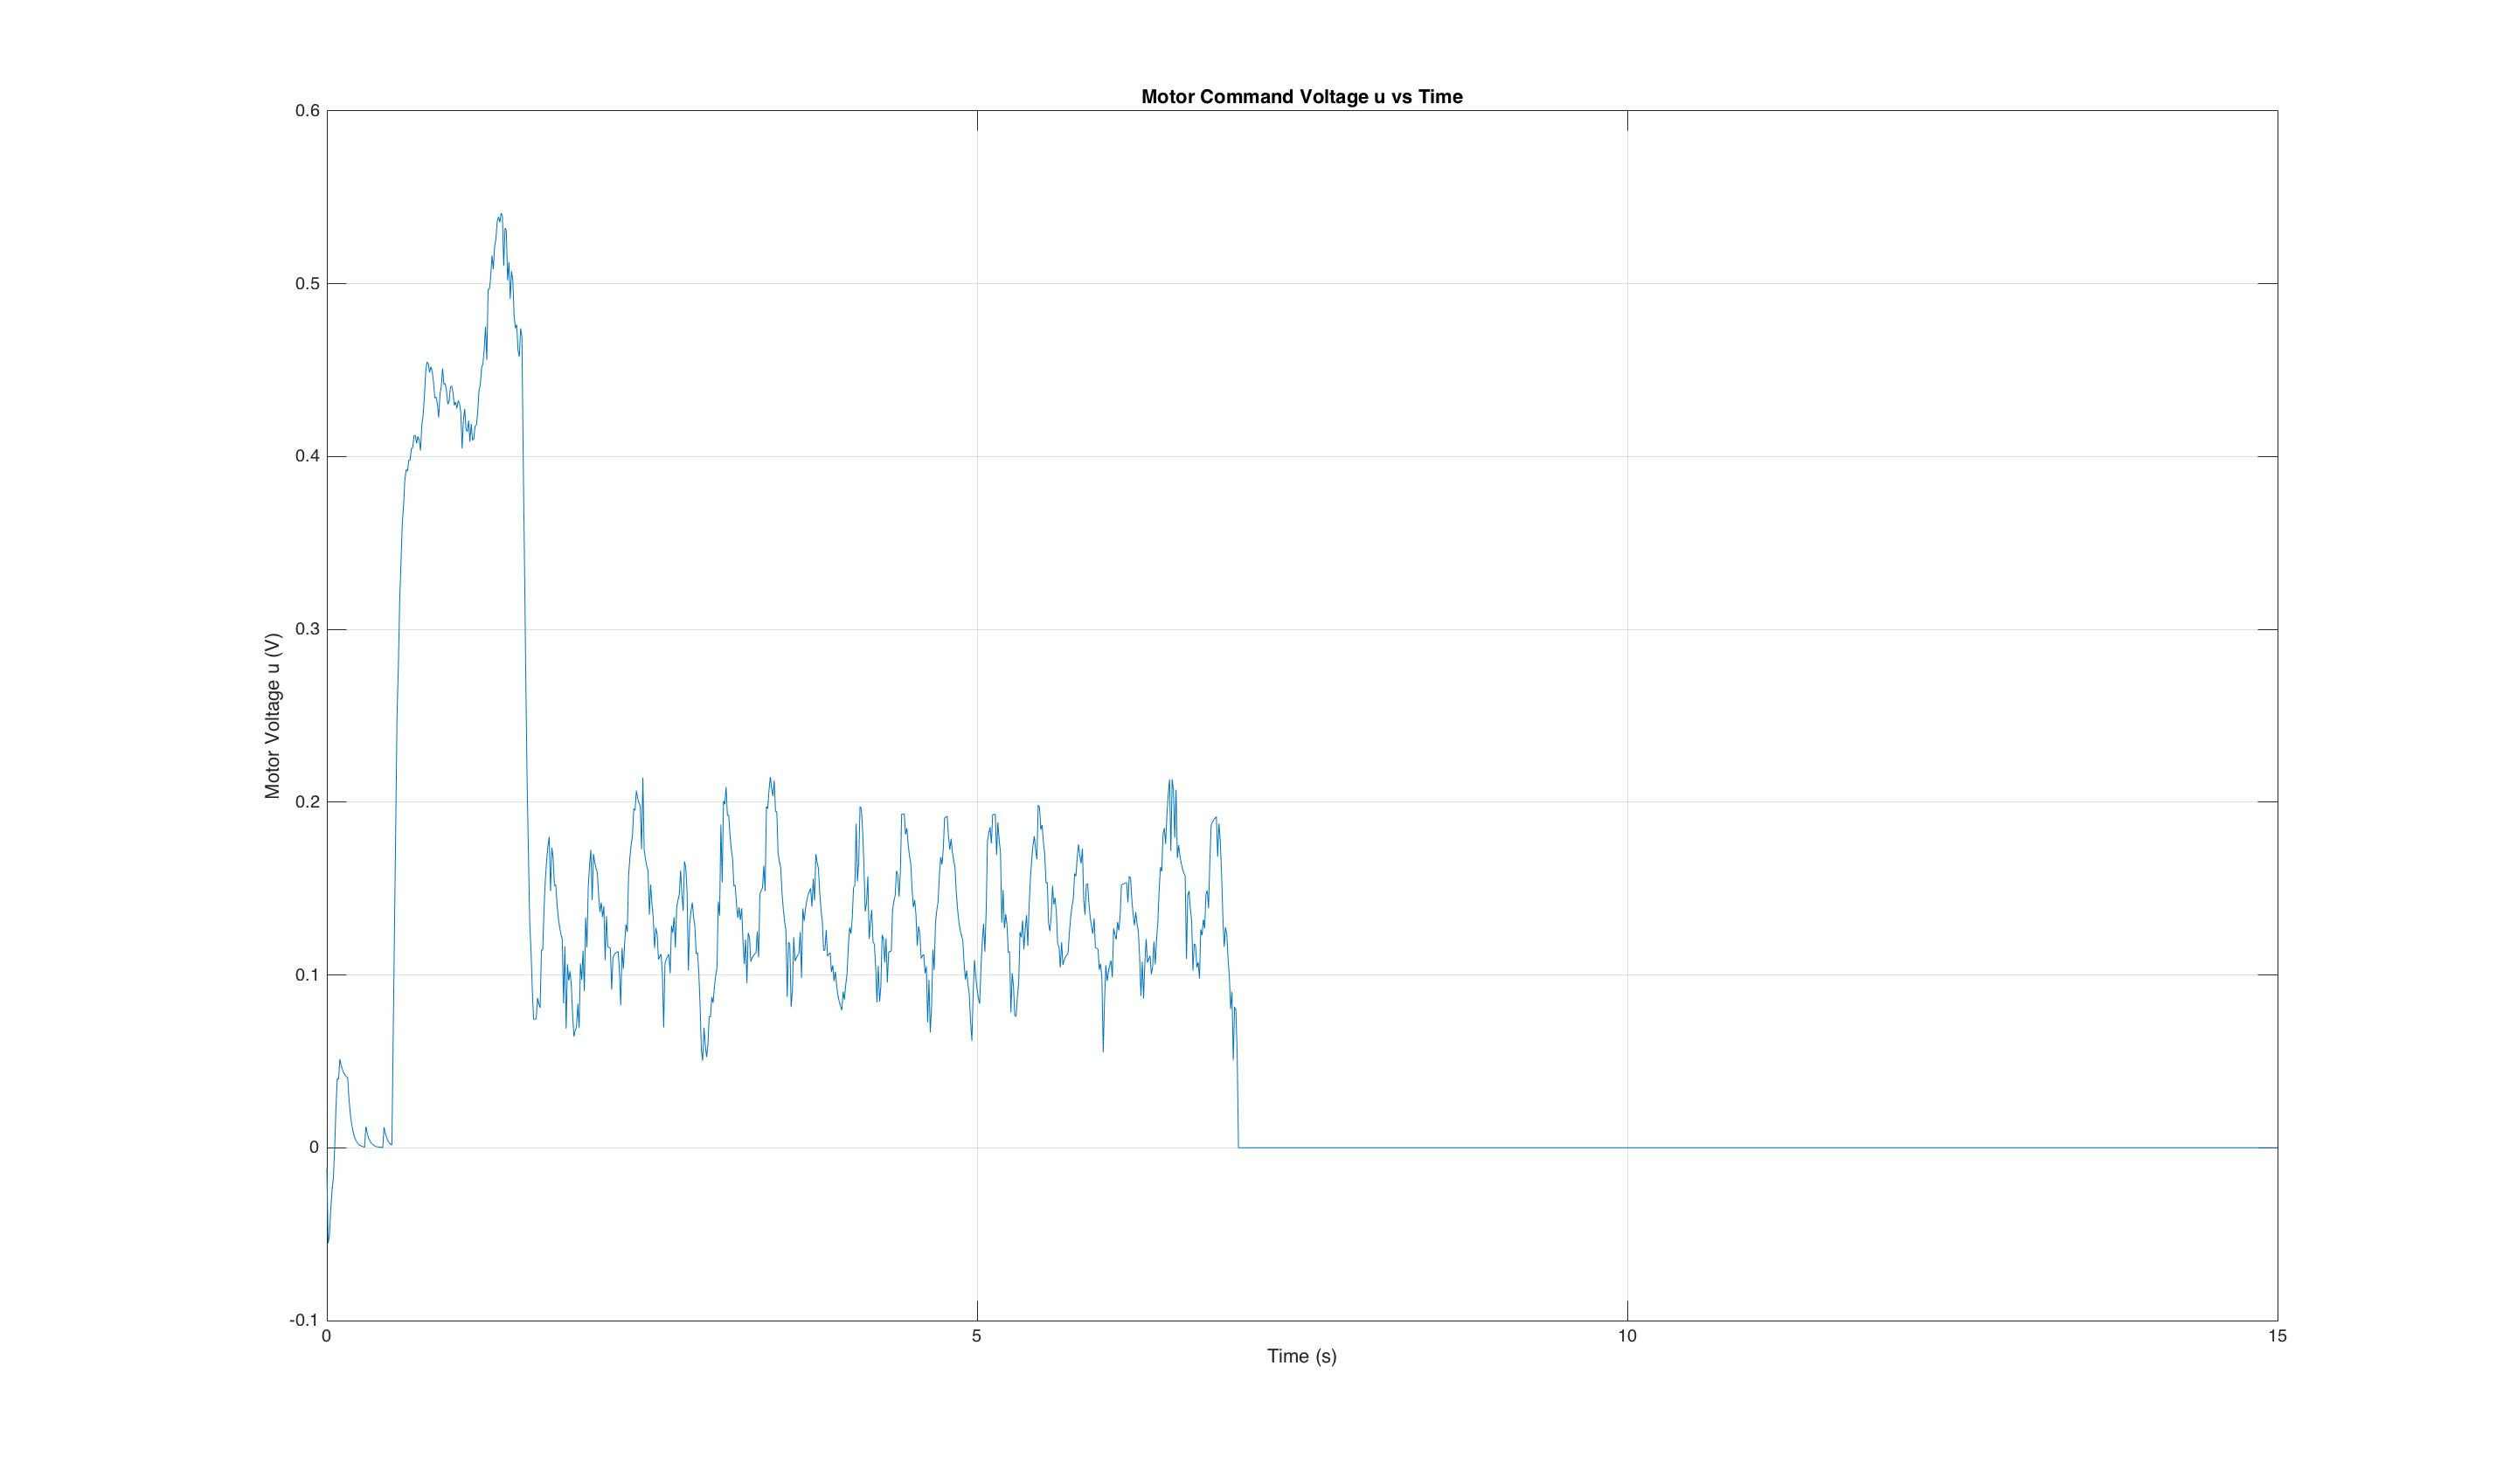
\includegraphics[scale=0.1]{u_vs_time}
            \caption{Motor Voltage $u$ vs. Time}
            \label{fig:u_vs_time}
        \end{figure}
    
\section{Introducing sinusoid to reference}
    \subsection{Frequency response and Bode analysis}
        With proportional control $k_p$, we see that the closed-loop transfer function of our system is 
        \begin{equation}
            H(s)=\frac{\frac{k_pk}{J}}{s+\frac{c+k_pk}{J}}
        \end{equation}
        Substituting our values for $k_p$ and $c$ in the system, for a gain of $k=1$, and an arrangement of 4 masses at 9 cm from the center of the disc ($J = 0.0192$), the transfer function becomes 
        \begin{equation}
            H(s)=\frac{18.74}{s + 19.15}
        \end{equation}
        A Bode plot of the system transfer function is shown in figure \ref{fig:bode_Hs}. The bandwidth of the system is determined from the Bode plot to be 19.015 Hz.
        \begin{figure}[h!]
            \centering
            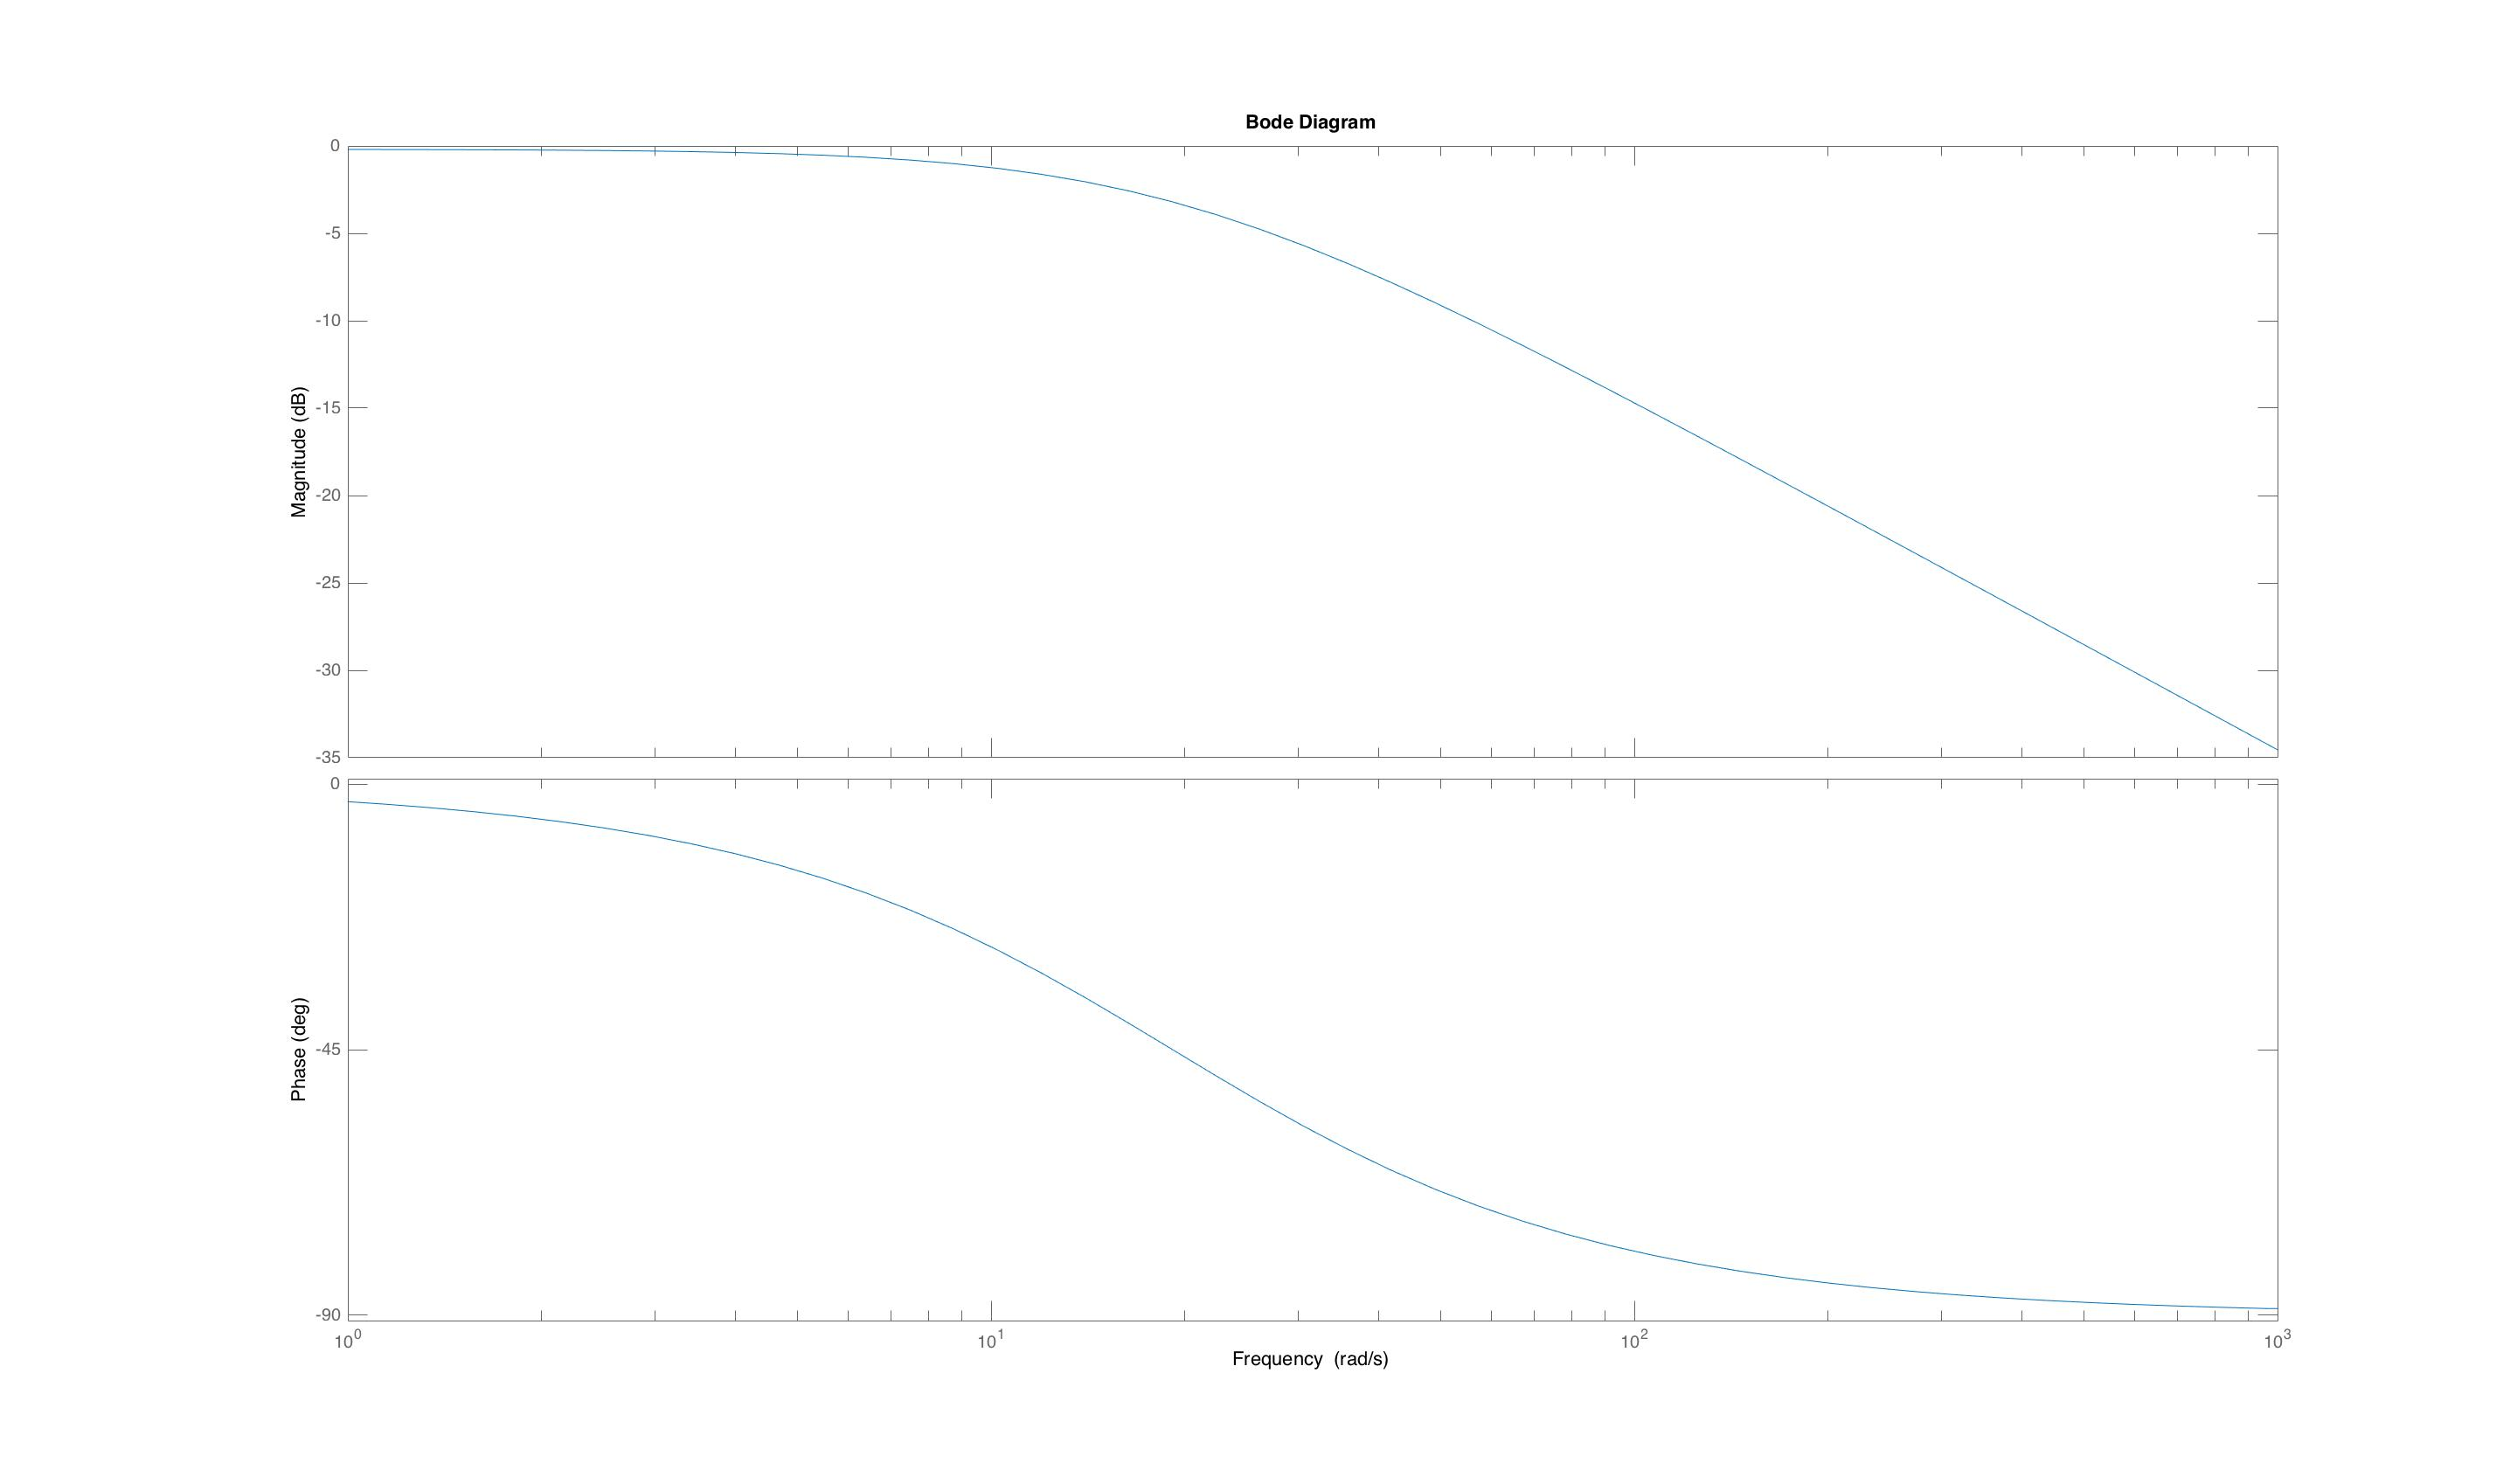
\includegraphics[scale=0.15]{bode_Hs}
            \caption{Bode Plot of System Transfer Function $H(s)$}
            \label{fig:bode_Hs}
        \end{figure}
    \subsection{System response to sinusoidal input}
        A sinusoidal input can be introduced to the system to further investigate the frequency response and time/phase delay of the system. For the LTI model, the introduction of a time delay results in the system equation 
        \begin{multline}
            J(\omega b_{\omega}cos(\omega t)-\omega a_{\omega}sin(\omega t)+c(a_{\omega}cos(\omega t)+b_{omega}sin(\omega t))\\
            = a_ucos(w(t-T_D))+b_usin(w(t-T_D))
        \end{multline}
        This representation of the system is explored in more detail in the third data collection experiment, which was conducted with the power connected to the Torsion Disc system and a sinusoidal reference input $\delta V_{ref}=2sin\pi ft$ added to the constant reference input. In this case the values of system parameters $k_p$ and $f$ are adjusted in LabView while the weights remain in the same position. The collected data is then used to investigate frequency response of the system.
    \subsection*{Steps}
        \begin{enumerate}
            \itemsep0em 
            \item set reference speed to 6.28 rad/sec
            \item set disturbance to 0
            \item set $K_p$ to 1
            \item adjust experiment length to 15 seconds in order to collect data as the system comes to a stop
            \item \textbf{Ensure there is someone with their finger on the power of button in case the system goes unstable}
            \item turn the power on
            \item press the run button in LabView, data is saved as a text file
            \item rename file to reflect parameter values
            \item repeat for the values listed in below table
        \end{enumerate}
        \begin{table}[h!]
            \centering
            \begin{tabular}{|m{4cm}|m{3cm}|m{3cm}|} 
                \hline
                Reference rad/sec & $K_p$ & Frequency \\ 
                \hline
                6.28 & 0.5 & 4Hz \\
                \hline
                6.28 & 1 & 5Hz\\
                \hline
            \end{tabular}
            \caption{Frequency Response Parameters} \label{table:freq_param}
        \end{table}
        From further experimentation with the system, we found that increasing the frequency of our input sinusoid above the bandwidth of the system did not cause the expected roll-off in amplitude even with a slight increase in $k_p$. For values of $k_p > 5$ the input motor voltage was saturated, suggesting additional dynamics at play in our system.
    \subsection{Fourier fit of sinusoidal input and response}   
        The sinusoidal input for motor voltage $u$ and output for rotational velocity $\omega$ can be graphically fit using fourier series, and the fourier coefficients can be obtained from this nonlinear curve fitting. Below the data for $u$ and $\omega$ are plotted (data points) along with their best fit sinusoids (blue line) for $k_p=1$ and $f=5$Hz.
        \begin{figure}[H]
            \centering
            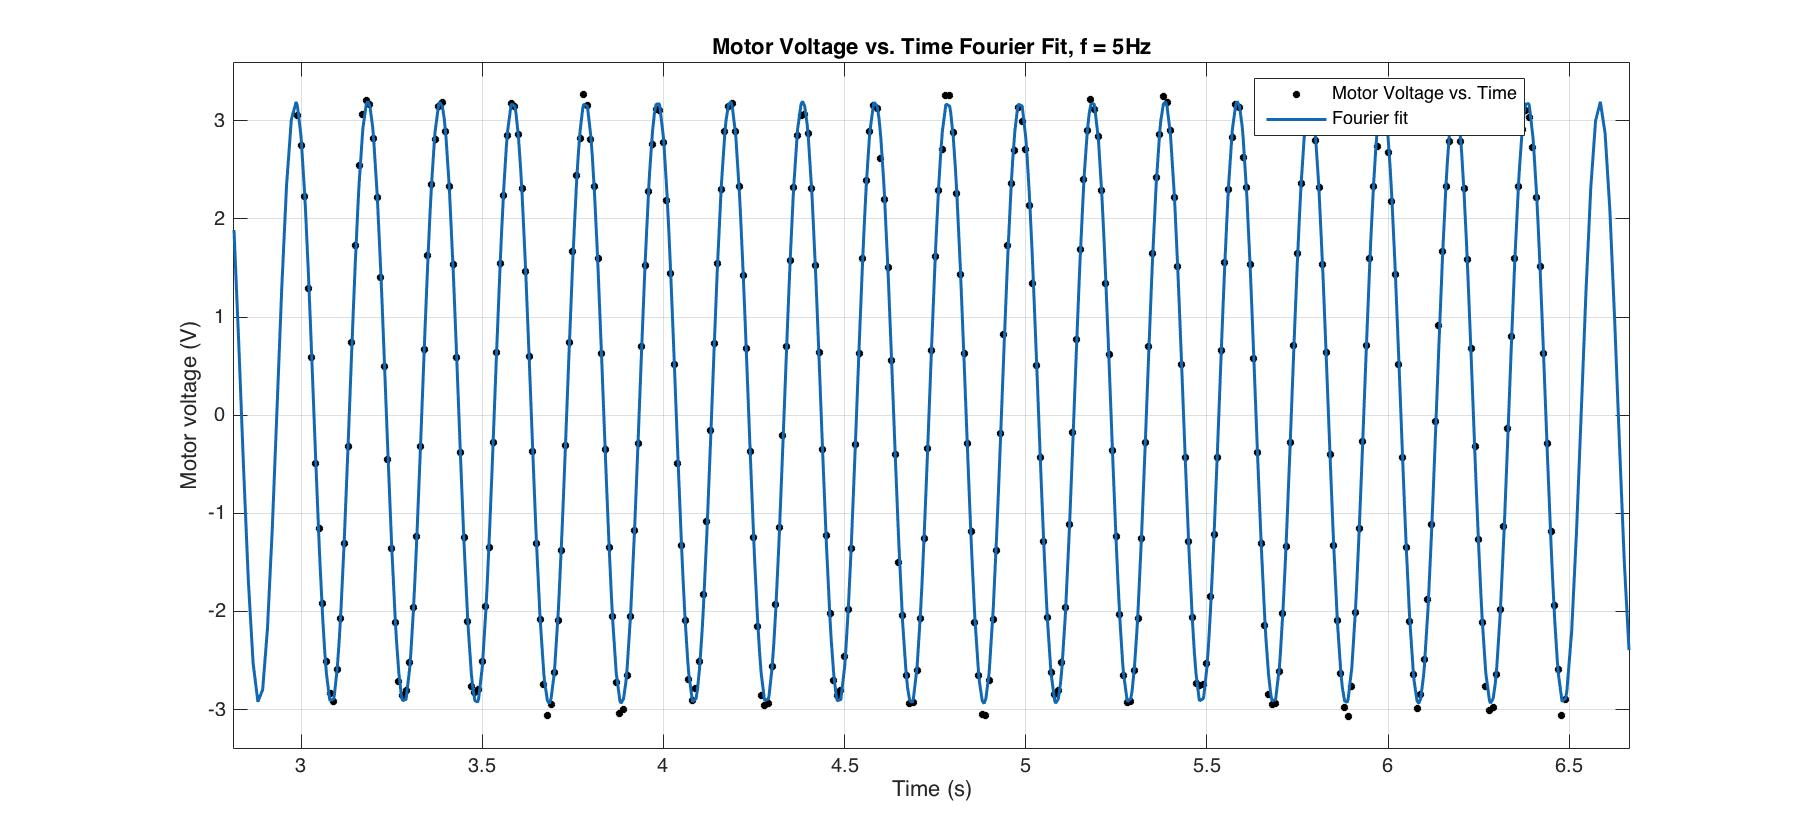
\includegraphics[scale=0.25]{fourier_volt_5Hz}
            \caption{Fourier Fit of Motor Command Voltage $u$}
            \label{fig:fourier_volt_5Hz}
        \end{figure}
        \begin{figure}[H]
            \centering
            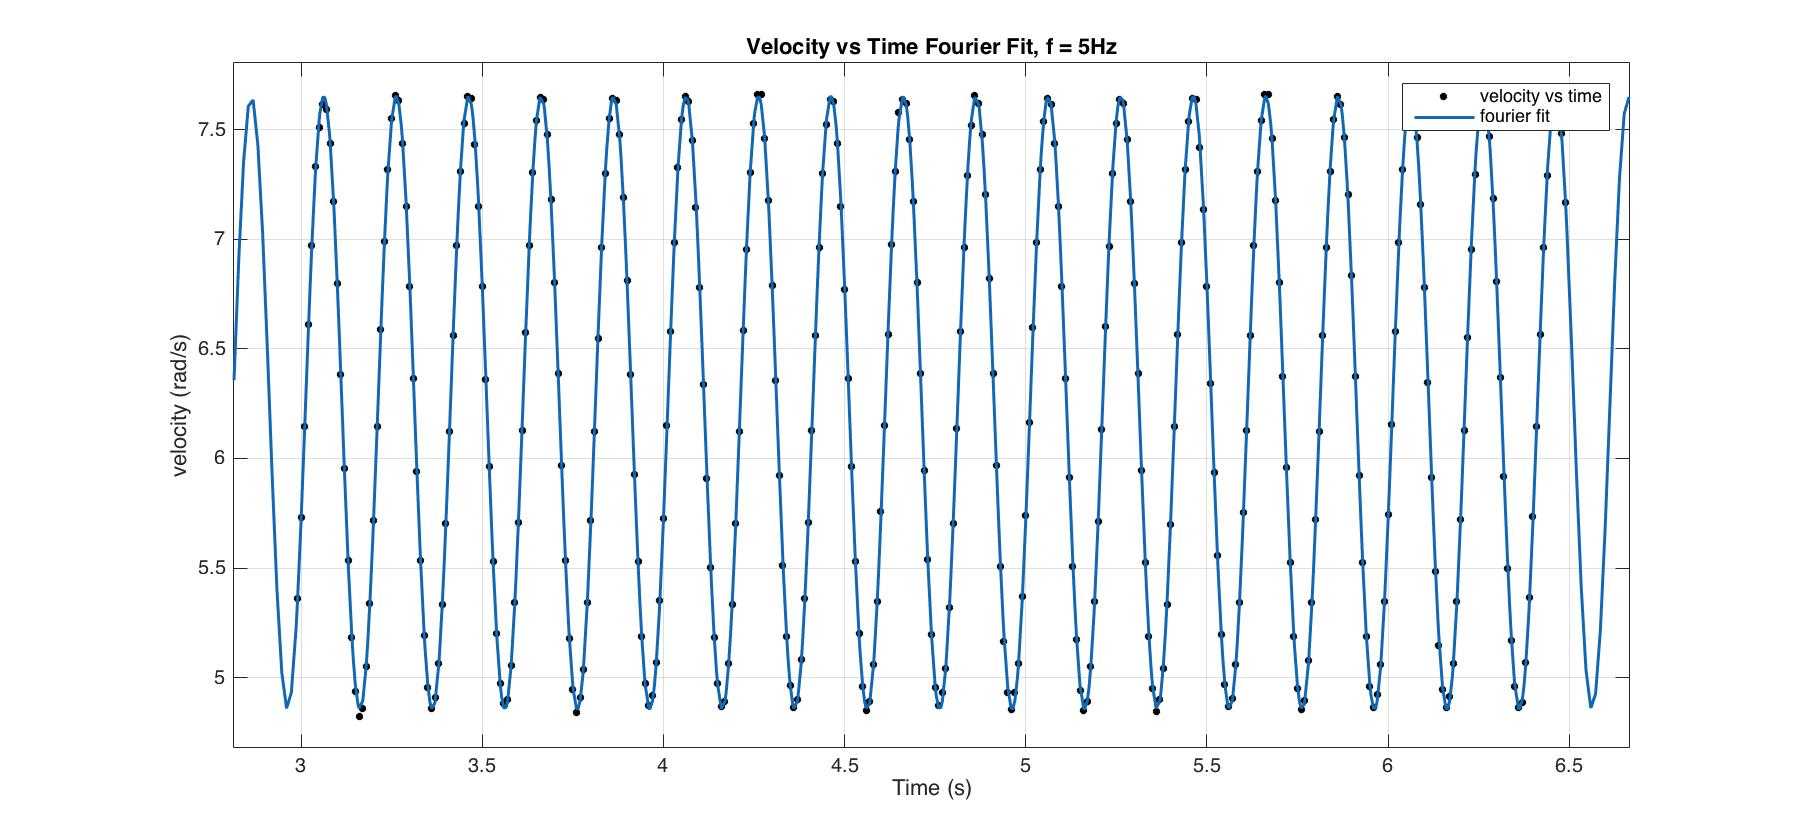
\includegraphics[scale=0.25]{fourier_vel_5Hz}
            \caption{Fourier Fit of Rotational Velocity $\omega$}
            \label{fig:fourier_vel_5Hz}
        \end{figure}
        \noindent The fourier coefficients obtained from the sinusoidal curve fitting are
        \begin{equation}
            a_{\omega}=-0.5444\hspace{0.5cm}b_{\omega}=1.289\hspace{0.5cm}a_u=2.712\hspace{0.5cm}b_u=-1.435\nonumber
        \end{equation}
        \noindent Inserting the above parameters into the fourier form of our LTI system equation, and separating into sine and cosine parts, we get
        \begin{align}
            J\omega b_{\omega}(\omega)+ca_{\omega}(\omega)&=k(a_u(\omega)cos(\omega T_D)-b_u(\omega)sin(\omega T_d)\\
            J\omega 1.289+(-0.544)c&=k(2.712cos(\omega T_D)+1.435sin(\omega T_d))
        \end{align}
        The time delay $T_D$ is estimated to be on the order of several hundredths of a second. Time delay and its impact on system stability will be examined in further experiments involving the torsion disc system. 
\section{Proportional Controller Design}
    The proportional controller for the torsion disc cruise control system must provide a relatively fast response, minimal overshoot, little error in steady state when tracking a constant velocity reference input, and some small finite error in disturbance rejection as well, so that bumps and hills do not greatly affect the system's performance. These objectives suggest a relatively large value for $k_p$, such as $k_p=10$, which was found to reduce instability and motor noise during experimentation with the system. However, when a non-constant input - such as a sinusoid - is introduced to the system, it was discovered that a much smaller value of $k_p$ was desired to avoid motor voltage saturation and to keep the system stable. If non-constant inputs are expected, then a smaller value of $k_p$, $k_p\leq1$ is desired. Thus, the best design for the proportional controller depends largely on the expected reference and disturbance inputs for a system. Beyond finding the best possible proportional gain for the system, we should investigate other methods of control. The introduction of integral control should provide more control over various aspects of the system, better steady state error and disturbance rejection, and a more robust system overall. PI control will be examined further for this system in the next set of experiments. 

\end{document}
